\chapter{Schleifen und Arrays}

\section{Schleifen}

Mit dem bisher gelernten Wissen sollte folgende Aufgabe für dich leicht zu lösen sein: Schreibe ein Programm, das die Zahlen von 1 bis 12 ausgibt. Etwas schwieriger wird die Aufgabe, wenn du die Zahlen von 1 bis einer Million ausgeben sollst oder die Obergrenze von einer Nutzereingabe abhängt. An dieser Stelle kommen Schleifen ins Spiel: Sie führen einen Anweisungsblock solange aus, bis eine bestimmte Bedingung erfüllt (oder nicht mehr erfüllt) ist. Java kennt, wie viele andere Programmiersprachen auch drei verschiedene Arten von Schleifen: Die \textit{for}-Schleife, die \textit{while}-Schleife und die \textit{do-while}-Schleife.

\subsection{Die FOR-Schleife}

Diese Schleife ist die, die man vermutlich am häufigsten sieht. Im Struktogramm wird sie wie in Abbildung \ref{for} verwendet.

\begin{figure}
	\begin{center}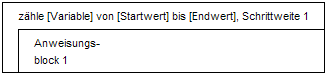
\includegraphics[scale=1]{images/for.png}\end{center}
	\caption{Die \textit{for}-Schleife in einem Struktogramm}
	\label{for}
\end{figure}

Für diese Art von Schleife braucht man eine explizite Laufvariable, die man inkrementieren kann. Im einfachsten Fall kann man dafür einen Integer benutzen. Das untenstehende Codebeispiel verdeutlicht die Benutzung einer \textit{for}-Schleife in Java.

\begin{minipage}{\textwidth}
\begin{lstlisting}
public class ForSchleife {
  public static void main(String[] args) {
    for(int i = 1; i <= 12; i=i+1){
      System.out.println(i);
    }
  }
}
\end{lstlisting}
\end{minipage}

Eine \textit{for}-Schleife braucht drei Informationen über die Laufvariable: Ihren Initialwert, hier mit \textit{int i = 1} geschehen, einen bool'schen Ausdruck wann die Schleife abbrechen soll, hier mit $i <=12$ angegeben. Das bedeutet, dass die Schleife nicht mehr ausgeführt wird, sobald $i$ diese Bedingung nicht mehr erfüllt, also 13 erreicht.

Am Ende benötigt man noch eine Aktion, die nach jedem Schleifendurchlauf gemacht werden soll, in diesem Fall wird mit \textit{i=i+1} die Laufvariable nach jedem Schleifendurchlauf inkrementiert.

\subsection{Die WHILE-Schleife}

Der Unterschied zu der \textit{for}-Schleife ist im Wesentlichen, dass keine konkrete Initialisierung benötigt und auf eine Behandlung der Variable nach jedem Schleifendurchlauf verzichtet wird. Im Struktogramm hat die \textit{while}-Schleife auch eine eigene Abbildung (\ref{while}).

\begin{figure}
	\begin{center}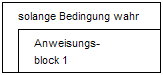
\includegraphics[scale=1]{images/while.png}\end{center}
	\caption{Eine \textit{while}-Schleife in einem Struktogramm}
	\label{while}
\end{figure}

In Java definiert der folgende Code eine \textit{while}-Schleife:

\begin{minipage}{\textwidth}
\begin{lstlisting}
public class IfThenElse {
  public static void main(String[] args) {
    int i = 1;
    while(i<=12){
      System.out.println(i);
      i = i+1;
    }
  }
}
\end{lstlisting}
\end{minipage}

Der Code hat den gleichen Effekt wie der bei der im letzten Abschnitt gezeigten \textit{for}-Schleife. Die Initialisierung findet hier jedoch vor der Schleife statt; die Inkrementierung der Variable findet in der Schleife statt.

\subsection{Die DO-WHILE Schleife}

Diese Schleife unterscheidet sich nicht wesentlich von der \textit{while}-Schleife. Im Gegensatz zu dieser wird die Bedingung aber erst am Ende geprüft und nicht am Anfang. Auch diese Schleife hat eine Entsprechung in einem Struktogramm (Abbildung \ref{dowhile}.

\begin{figure}
	\begin{center}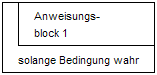
\includegraphics{images/dowhile.png}\end{center}
	\caption{Die \textit{do-while}-Schleife in einem Struktogramm}
	\label{dowhile}
\end{figure}

Der Javacode ähnelt ebenfalls sehr der \textit{while}-Schleife:

\begin{minipage}{\textwidth}
\begin{lstlisting}
public class IfThenElse {
  public static void main(String[] args) {
    int i = 1;
    do{
      System.out.println(i);
      i = i+1;
    }while(i<=12);
  }
}
\end{lstlisting}
\end{minipage}

Diese Schleife läuft also, unabhängig davon ob die Bedingung am Anfang erfüllt ist oder nicht, mindestens ein mal durch.

\subsection{Gefahren von Schleifen}

Jeder Code, den du bisher geschrieben hast, läuft bei korrekter Syntax durch und das Programm wird irgendwann beendet sein. Bei Schleifen ist diese Tatsache nicht mehr garantiert. Der folgende Code hat zwar eine völlig korrekte Syntax, wird aber bei der Ausführung eine niemals terminierende Endlosschleife sein:

\begin{minipage}{\textwidth}
\begin{lstlisting}
public class IfThenElse {
  public static void main(String[] args) {
    int i = 1;
    while(i<=12){
      System.out.println(i);
    }
  }
}
\end{lstlisting}
\end{minipage}

Hier wurde vergessen, die Variable, die in der Bedingung geprüft wird, zu ändern. Die Bedingung \textit{$i\le 12$} wird damit immer wahr sein und damit wird die Schleife nie verlassen. Wenn ihr also ein Programm schreibt, es laufen lasst und es hört einfach nicht auf zu rechnen, dann ist es möglicherweise solche eine Endlosschleife die das Problem erzeugt. Es ist eure Aufgabe als Programmierer, darauf zu achten das jede Schleife terminiert.

Im letzten Kapitel hast du bereits das Schlüsselwort \textit{break;} kennengelernt. Es wurde dazu verwendet um sofort aus einer \textit{switch}-Anweisung herauszuspringen. Ein \textit{break;} in einer Schleife hat die gleiche Funktion: Die Ausführung der Schleife wird sofort beendet und der Code wird nach der Schleife fortgesetzt.

\begin{minipage}{\textwidth}
\begin{lstlisting}
public class IfThenElse {
  public static void main(String[] args) {
    for (int i = 1; i <= 12; i++){
      System.out.println(i);
      if (i==6){
        break;
      }
    }
    System.out.println("Nach der Schleife");
  }
}
\end{lstlisting}
\end{minipage}

Das Ergebnis des obenstehenden Codes ist, dass nur die Zahlen von eins bis sechs ausgegeben werden und die Schleife danach mittels des \textit{break;} verlassen wird, unabhängig von dem Wahrheitswert der Abbruchbedingung der Schleife. 

Für Schleifen gibt es noch ein zweites derartiges Schlüsselwort: \textit{continue;}. Im Gegensatz zu \textit{break;} bricht es nicht die komplette Schleife ab sondern lediglich den aktuellen Schleifendurchlauf. Der untenstehende Code wird also alle Zahlen zwischen eins und zwölf ausgeben außer der 6:

\begin{minipage}{\textwidth}
\begin{lstlisting}
public class IfThenElse {
  public static void main(String[] args) {
    for (int i = 1; i <= 12; i++){
      if (i==6){
        continue;
      }
      System.out.println(i);
    }
    System.out.println("Nach der Schleife");
  }
}
\end{lstlisting}
\end{minipage}

\subsection{Aufgaben}

\begin{enumerate}
	\item Implementiere eine Schleife, die eine Integer-Zahl von der Konsole liest und alle natürlichen Zahlen kleiner oder gleich der gelesenen Zahl ausgibt. Implementiere das Programm mit Hilfe einer
	\begin{itemize}
		\item \textit{for}-Schleife
		\item \textit{while}-Schleife
		\item \textit{do-while}-Schleife
	\end{itemize}
	\item Verändere das Programm mit der \textit{for}-Schleife, sodass es nur noch die geraden Zahlen ausgibt. Verändere dabei
	\begin{itemize}
		\item nur den Anweisungsblock in der Schleife.
		\item nur den Schleifenkopf.
	\end{itemize}
	\item Schreibe ein Programm das von der Konsole zwei Integer $n$ und $m$ liest. Gib alle Zahlen zwischen $1$ und $n\cdot m$ in n Spalten und m Zeilen ausgibt. (Hinweis: Es ist möglich eine Schleife in einer Schleife zu definieren)
	\item Schreibe ein Programm das für eine eingegebene Zahl prüft, ob sie eine Primzahl ist. (Hinweis: Das Sieb des Eratosthenes bietet einen möglichen Algorithmus)
	\item Schreibe ein Programm welches alle Primzahlen bis zu einer von dem Nutzer eingegebenen Obergrenze ausgibt.
\end{enumerate}

\section{Arrays}

Du weißt bereits was Variablen und Datentypen sind. Wenn man beispielsweise die Höchsttemperatur eines Tages speichern möchte, kann man sich dafür ein \textit{double} deklarieren, in dem man diesen Wert speichern kann. Jetzt könnte man zum Beispiel die Aufgabe bekommen, die Höchsttemperaturen von jedem Tag der Woche zu speichern. Man kann dafür natürlich 7 Variablen anlegen. Wenn man den Zeitraum für das Speichern der Temperaturen aber ausweitet, zum Beispiel auf ein Jahr, dann kann auch das anstrengend werden.

Arrays sind ein Weg um die Speicherung solcher gleichartigen Datenmengen einfach umzusetzen. Man kann sich ein Array wie eine lange Reihe von Schließfächern vorstellen: in jedem Schließfach gibt es einen Inhalt, und mit der Nummer des Schließfachs kann man auf den Inhalt zugreifen. Die Verwendung von Arrays in Java zeigt das folgende Codebeispiel:

\begin{minipage}{\textwidth}
\begin{lstlisting}
public class IfThenElse {
  public static void main(String[] args) {
    double[] temperature = new double[365];
    temperature[42] = 13.37;
    System.out.println(temperature[42]);
    System.out.println(temperature[23]);
  }
}
\end{lstlisting}	
\end{minipage}

In der ersten Zeile wird der Container deklariert: Es wird Platz für 365 \textit{double}-Werte reserviert und jeder der Werte wird mit einem Standardwert, in diesem Fall $0.0$, initialisiert. In der zweiten Zeile befülle ich den 42. Platz des Containers mit einem Wert: $13.37$, der in der dritten Zeile wieder ausgegeben wird. Die Ausgabe in der vierten Zeile wird $0.0$ ausgeben, da kein anderer Wert diesem Container zugewiesen wurde.

\begin{itemize}
	\item[\textit{Bemerkung:}] Die Initialisierung mit einem Standardwert ist eine Eigenheit von Java. Viele andere Programmiersprachen, zum Beispiel C++, würden an dieser Stelle einen (mehr oder weniger) zufälligen Wert zurückgeben.
\end{itemize}

Ähnlich wie das Schachteln von Schleifen, können auch Arrays ''geschachtelt'' werden. Wenn man sich ein eindimensionales Array als Reihe eines Schachbretts vorstellt, dann ist das komplette Brett ein zweidimensionales Array. Ein dreidimensionales Array kann man sich als viele Schachbretter übereinander vorstellen. Die Vorstellung von Dimensionen größer als drei überlasse ich an der Stelle lieber den Mathematikern. Die Deklaration eines mehrdimensionalen Arrays kann wie folgt aussehen:

\begin{minipage}{\textwidth}
\begin{lstlisting}
public class IfThenElse {
  public static void main(String[] args) {
    String[][] chessBoard = new String[8][8];
  }
}
\end{lstlisting}	
\end{minipage}

Natürlich muss man auch bei Arrays auf Dinge achten. So kann man in Java bei einem Array, das mit $n$ Feldern initialisiert wurde auf die Felder $0$ bis $n-1$ zugreifen. Ein Zugriff auf einen Wert außerhalb dieses Bereichs führt zu einem Absturz des geschriebenen Programms. Ein weiterer Nachteil von Arrays ist es, dass man eine Größe beim Programm spezifizieren muss. Datenstrukturen, die diesen Nachteil umgehen wirst du im Laufe des ersten Semesters kennenlernen.

Eine häufig genutzte Funktion von Arrays ist das bestimmen der Größe um zum Beispiel die Anzahl der Schleifendurchläufe zu bestimmen:

\begin{minipage}{\textwidth}
\begin{lstlisting}
public class IfThenElse {
  private const int ARRAY_SIZE = 8;
  public static void main(String[] args) {
    int[] example = new int[ARRAY_SIZE];
    for (int i = 0; i < example.length; i++{
      //do something
    }
  }
}
\end{lstlisting}	
\end{minipage}

Insbesondere beim Einlesen der Größe des Arrays, wenn man also die Größe des Arrays nicht von vornherein kennt, ist diese Funktion sehr hilfreich.

\subsection{Aufgaben}

\begin{enumerate}
	\item Schreib ein Programm, das für ein Array von Integern oder Floats die Summe aller ihrer Elemente ausgibt.
	\item Schreib ein Programm, welches zwei gleich große Arrays von Integern oder Floats entgegennimmt und die Elementweise Summe in ein neues Array schreibt.
	\item Schreib ein Programm, welches die Größe eines zu erstellenden Arrays vom Nutzer einliest. Fülle dieses Array der Größe $n$ mit den ersten $n$ Primzahlen.
	\item Spieglein, Spieglein in meinem Programm, spiegle ein Zweidimensionales Array. (Es sollen sich also die Werte an anderen Stellen wiederfinden.
	\item Schreib ein Programm, in dem zu jeder Person mehrere schlechte Wortwitze abgespeichert werden können. Was wäre eine Wortspielkasse, ohne ein tolles Javaprogamm?
\end{enumerate}

